
% This LaTeX was auto-generated from MATLAB code.
% To make changes, update the MATLAB code and republish this document.

\documentclass{article}
\usepackage{graphicx}
\usepackage{color}

\sloppy
\definecolor{lightgray}{gray}{0.5}
\setlength{\parindent}{0pt}

\begin{document}

    
    
\subsection*{Contents}

\begin{itemize}
\setlength{\itemsep}{-1ex}
   \item Soft Margin SVN vs Loss function-minimizing hyperplane
   \item Plotting the classifier
   \item Implementing Stochastic Gradient Descent
\end{itemize}


\subsection*{Soft Margin SVN vs Loss function-minimizing hyperplane}

\begin{par}
Recall that the soft margin problem is as follows:
\end{par} \vspace{1em}
\begin{par}

\begin{align}
\text{min}&\frac{1}{2}||w||^2 + C\sum_{i=1}^{n}\xi_i \, \text{w.r.t} \\
&y_i(w^{\top}x_i + b) \geq 1 - \xi_i
\end{align}

\end{par} \vspace{1em}
\begin{par}
The corresponding dual problem is
\end{par} \vspace{1em}
\begin{par}
\begin{verbatim}latex\end{verbatim} \ensuremath{\backslash}begin\{align\} \ensuremath{\backslash}text\{min\}\&\ensuremath{\backslash}frac\{1\}\{2\}D'\ensuremath{\backslash}lambda - [1\_\{1\ensuremath{\backslash}times n\} 0\_\{1\ensuremath{\backslash}times n\}]\ensuremath{\backslash}lambda\ensuremath{\backslash}, \ensuremath{\backslash}text\{w.r.t\}\ensuremath{\backslash}\ensuremath{\backslash} \& C \ensuremath{\backslash}geq \ensuremath{\backslash}lambda\_i \ensuremath{\backslash}geq 0 \ensuremath{\backslash}, 1 \ensuremath{\backslash}leq i \ensuremath{\backslash}leq 2n \ensuremath{\backslash}\ensuremath{\backslash} \& \ensuremath{\backslash}sum\_\{i=1\}\^{}\{n\}\ensuremath{\backslash}lambda\_iy\_i = 0 \ensuremath{\backslash}\ensuremath{\backslash} \& \ensuremath{\backslash}lambda\_i + \ensuremath{\backslash}lambda \_\{i+n\} = C \ensuremath{\backslash}, 1 \ensuremath{\backslash}leq i \ensuremath{\backslash}leq n \ensuremath{\backslash}end\{align\}
\end{par} \vspace{1em}
\begin{verbatim}
%</latex>
%
% Here $\lambda \in \mathbb{R}^{2n}$, $D' =
% \begin{bmatrix}(yy^{\top})\odot(XX^{\top}) & \\ & 0_{n\times
% n}\end{bmatrix}$. We can eliminate the equality constraint
% $\lambda_i + \lambda _{i+n} = C$ by setting
% $\lambda _{i+n} = C - \lambda_i$ and combining it with non-negativity
% to get $C \geq \lambda_i$ for $1 \leq i \leq n$.
% We can thus drop to solving for the first $n$ $\lambda$; the initial
% guess is $\lambda = 0_{n \times 1}$ and all the constraints are active.
% We also set the penalty constant $C$ to be $0.1$.
\end{verbatim}
\begin{par}
Setting up arguments for ASM.m
\end{par} \vspace{1em}
\begin{verbatim}
c = 0.2; %Constant in the penalty function
y = label; % the label vector
n = length(y); % number of data points
%D = [(y*y').*((XX * XX')) zeros(n,n); zeros(n,n) zeros(n,n)]; %SPD matrix
%                                                              in quadratic
%                                                              program
D = (y*y').*((XX * XX'));
%d = [ones(n,1); zeros(n,1)]; % linear term in Q.P
d = ones(n,1);
%Ap = [eye(n,n) eye(n,n)]; % the matrix A'
%App = [y' zeros(1,n)]; % the matrix A
App = y';
C = [eye(n,n); -eye(n,n); App];  %matrix of contraints
%b = [zeros(2*n + 1,1); c*ones(n,1)]; % vector of constraints
b = [zeros(n,1); -c*ones(n,1); 0];
gfun = @(x) D*x - d; %gradient
Hfun = @(x) D; %hessian
%init = [zeros(n,1); c*ones(n,1)]; % initial guess
init = zeros(n,1);
%W = [1:n (2*n + 1):(3*n + 1)]; %set of working constraints at the initial point
W = 1:n;
W = W';
% The constraints matrix is a 2n+1 by n matrix
% All constraints are active.
% Time to run the solver!
[lambs, lm] = ASM(init, gfun, Hfun, C, b, W);
soln = lambs(:,end); % extracting the lambda vector
wASM = (XX')*(y .* soln); % optimal w
%Computing B via soft margin support vectors
avg = XX(find(soln == max(soln(find(y==1)))),:) ...
    + XX(find(soln == max(soln(find(y==-1)))),:);
B = -0.5*(avg * wASM);
wASM = [wASM; B];
\end{verbatim}


\subsection*{Plotting the classifier}

\begin{verbatim}
% Plotting the data
idem = find(y==-1);
igop = find(y==1);
figure;
hold on; grid;
xmin = min(XX(:,1)); xmax = max(XX(:,1));
ymin = min(XX(:,2)); ymax = max(XX(:,2));
zmin = min(XX(:,3)); zmax = max(XX(:,3));
X1 = (XX(:,1)-xmin)/(xmax-xmin);
X2 = (XX(:,2)-ymin)/(ymax-ymin);
X3 = (XX(:,3)-zmin)/(zmax-zmin);
XX = [X1,X2,X3];
plot3(XX(idem,1),XX(idem,2),XX(idem,3),'.','color','b','Markersize',20);
plot3(XX(igop,1),XX(igop,2),XX(igop,3),'.','color','r','Markersize',20);
view(3)
fsz = 16;
set(gca,'Fontsize',fsz);
xlabel(str(i1),'Fontsize',fsz);
ylabel(str(i2),'Fontsize',fsz);
zlabel(str(i3),'Fontsize',fsz);

%Plotting the hyperplane

xmin = min(XX(:,1)); xmax = max(XX(:,1));
ymin = min(XX(:,2)); ymax = max(XX(:,2));
zmin = min(XX(:,3)); zmax = max(XX(:,3));
nn = 50;
[xx,yy,zz] = meshgrid(linspace(xmin,xmax,nn),linspace(ymin,ymax,nn),...
    linspace(zmin,zmax,nn));
plane = wASM(1)*xx+wASM(2)*yy+wASM(3)*zz+wASM(4);
plane2 = w(1)*xx+w(2)*yy+w(3)*zz+w(4);
p = patch(isosurface(xx,yy,zz,plane,0));
q = patch(isosurface(xx,yy,zz,plane2,0));
p.FaceColor = 'green';
p.EdgeColor = 'none';
q.FaceColor = 'red';
q.EdgeColor = 'none';
camlight
lighting gouraud
alpha(0.3);
%
\end{verbatim}

        \color{lightgray} \begin{verbatim}A local solution is found, iter = 351
x = [
0
2.000000e-01
1.931488e-15
2.000000e-01
2.000000e-01
2.000000e-01
2.000000e-01
2.000000e-01
-9.609228e-16
2.000000e-01
2.000000e-01
2.000000e-01
2.000000e-01
2.000000e-01
2.000000e-01
1.708555e-15
2.000000e-01
2.000000e-01
2.000000e-01
2.000000e-01
6.838316e-02
5.431399e-16
2.000000e-01
2.000000e-01
9.395453e-18
2.000000e-01
1.405835e-17
2.000000e-01
2.000000e-01
2.000000e-01
2.000000e-01
2.000000e-01
2.000000e-01
-7.658025e-16
2.000000e-01
2.000000e-01
2.000000e-01
2.000000e-01
2.000000e-01
2.000000e-01
3.246024e-16
2.000000e-01
-1.915655e-16
2.000000e-01
2.000000e-01
2.000000e-01
2.000000e-01
6.379186e-16
2.000000e-01
2.000000e-01
2.000000e-01
2.000000e-01
2.000000e-01
2.000000e-01
2.000000e-01
2.000000e-01
2.000000e-01
2.000000e-01
2.000000e-01
2.000000e-01
2.000000e-01
2.000000e-01
2.000000e-01
2.000000e-01
2.000000e-01
2.000000e-01
2.000000e-01
2.000000e-01
2.000000e-01
2.000000e-01
2.000000e-01
2.000000e-01
2.000000e-01
2.000000e-01
2.000000e-01
2.000000e-01
2.000000e-01
2.000000e-01
2.000000e-01
2.000000e-01
2.000000e-01
2.000000e-01
2.000000e-01
2.000000e-01
2.000000e-01
2.000000e-01
2.000000e-01
2.000000e-01
2.000000e-01
2.000000e-01
2.000000e-01
2.000000e-01
2.000000e-01
2.000000e-01
2.000000e-01
2.000000e-01
2.000000e-01
2.000000e-01
2.000000e-01
2.000000e-01
2.000000e-01
2.000000e-01
2.000000e-01
2.000000e-01
2.000000e-01
2.000000e-01
2.000000e-01
2.000000e-01
2.000000e-01
2.000000e-01
2.000000e-01
2.000000e-01
]
\end{verbatim} \color{black}
    
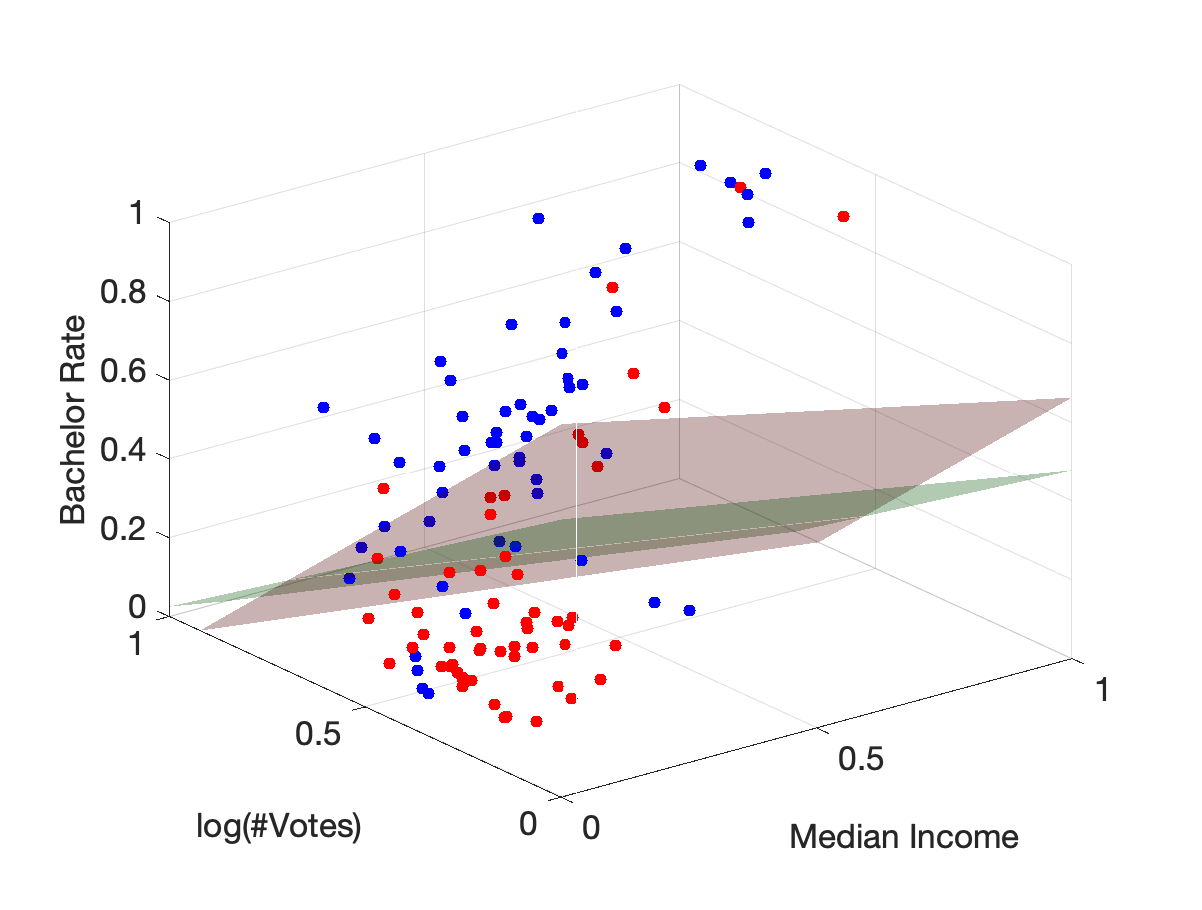
\includegraphics [width=4in]{Report_01.eps}


\subsection*{Implementing Stochastic Gradient Descent}

\begin{verbatim}
function SGD(init,grad,step,batch)
    % init--initial guess
    % grad--function that evaluates gradient of f at current iterate
    %
    N = 15;
    NN = 10;
    for ii = 1 : NN
    s = step/2^ii;
    nsteps = ceil(N*2^ii/ii);
    for i = 1 : nsteps
    k = randi(n);
    g = grad(k,x);
    x = x - g*s;
    end
    end
end
\end{verbatim}



\end{document}
    
